\section{Ways of Working}
\label{s:Ways-of-Working}
During the early stage of the project, many things needed to be decided, such as
the language, the agile framework, testing, and how to document everything. The
best agile frameworks that would be fit for purpose during the development
process were Kanban and Scrum. It is essential to have a good understanding of
how to work Agile. Agile is an approach very well known in the industry that
facilitates the management of a project by an individual or a group of
developers, designers and managers of the same team. It provides a rigorous
methodology, depending on which framework, to self-organise work and not deviate
from the end goal the team did impose themselves (or their company).
While working on this project, an Agile framework will be chosen and used as one
of the main requirements to simulate the working of a team of one or more,
working for a company or themselves. The goal is to have a simulated experience,
create a habit, and document the process, the decisions, and the steps taken
from the initial thoughts to the end product. Two main two frameworks will be
discussed and evaluated: Kanban and Scrum.

\section{Kanban vs Scrum}
\label{s:Kanban-vs-Scrum}
Scrum is fast and has ceremonies split into sprint planning, review,
retrospective, and daily standups. With Scrum, the team wants to ship a piece of
functionality by the end of each sprint and each sprint usually last two weeks.
Kanban on the other hand is much more flexible and based on continuous delivery
on the idea of having a backlog where the team can park their future work and
then move it next as soon as it is unblocked from other tickets. In Kanban new
feature and pieces of code are released when ready and one do not need to be too
worried of the deadlines given by the sprint such as in the Scrum framework.

\section{Agile Project Management}
\label{s:Agile-Project-Management}
As previously mentioned, there must always be a tool and techniques to keep
track of the work must has been done and the progress in general. For this
specific project, a Kanban board has been used to keep track of the work, while
still retaining some aspects of Scrum, which gives the framework a more flexible
approach that is more recognised as a Scrumban approach. Below an example of
tickets created in a Kanban board that makes it so visually appealing and easy
to work with.

\begin{figure}[H]
  \centering
  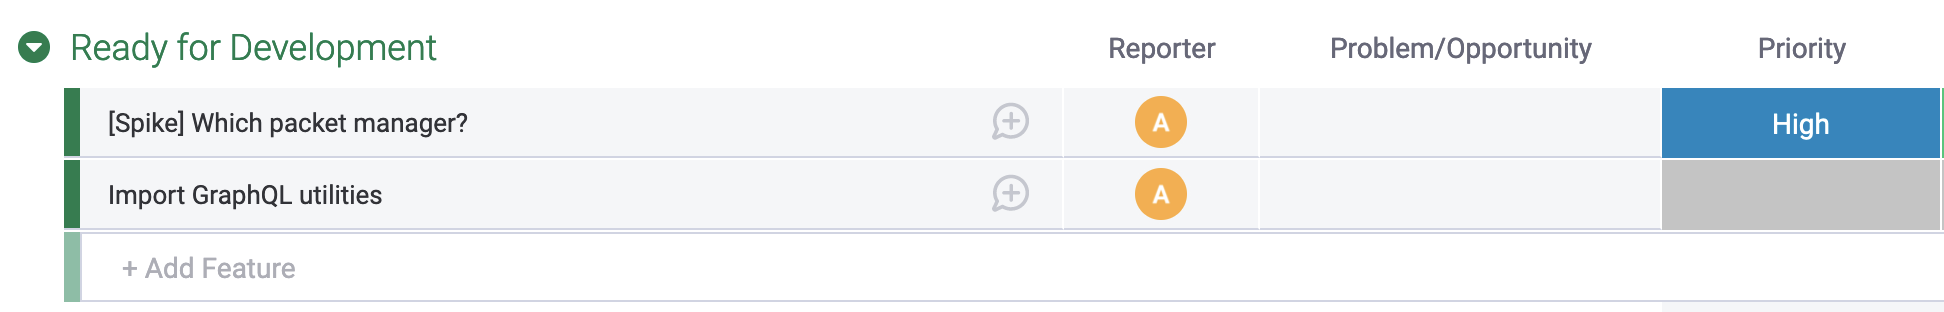
\includegraphics[width=1\textwidth]{figures/readyfordev}
  \caption{Ready for Development Agile Board}
  \label{f:readyfordev}
\end{figure}

The Ready for Development board is used for all the tickets that have been
through the whole initial lifecycle that comphrehend creation, refinement,
estimation, and ready to start. This approach is used throughout the project
cerimonies but for the sake of the speed have been reduced to a single
evaluation in the backlog as in this project there is only one working developer.

\subsection{Epics}
\label{s:Epic}
When a huge pieces of functionality needs more than a ticket, a new epic is created
where all the moving parts of the new functionality are put together. The epic
usually have a description that summarise the whole functionality, what needs
to be done to reach the end goal and the members involved.

\subsection{Spikes}
\label{s:Spikes}
When an investigation is required to find a solution which is unknown to the team,
a spike is created. A spike is a ticket that is used to gather information and
answering questions instead of producing a piece of functionality or solution.
The outcome of a spike is usually documented in the ticket itself and it usually
blocks other tickets from being moved to Ready to Developement. This project
has a spike for starting points such as language to use, tools, and frameworks.
